\documentclass{standalone}
\usepackage{tikz}
\usetikzlibrary{patterns, positioning}
\usepackage[sfdefault]{ClearSans} %% option 'sfdefault' activates Clear Sans as the default text font
\usepackage[T1]{fontenc}

\begin{document}
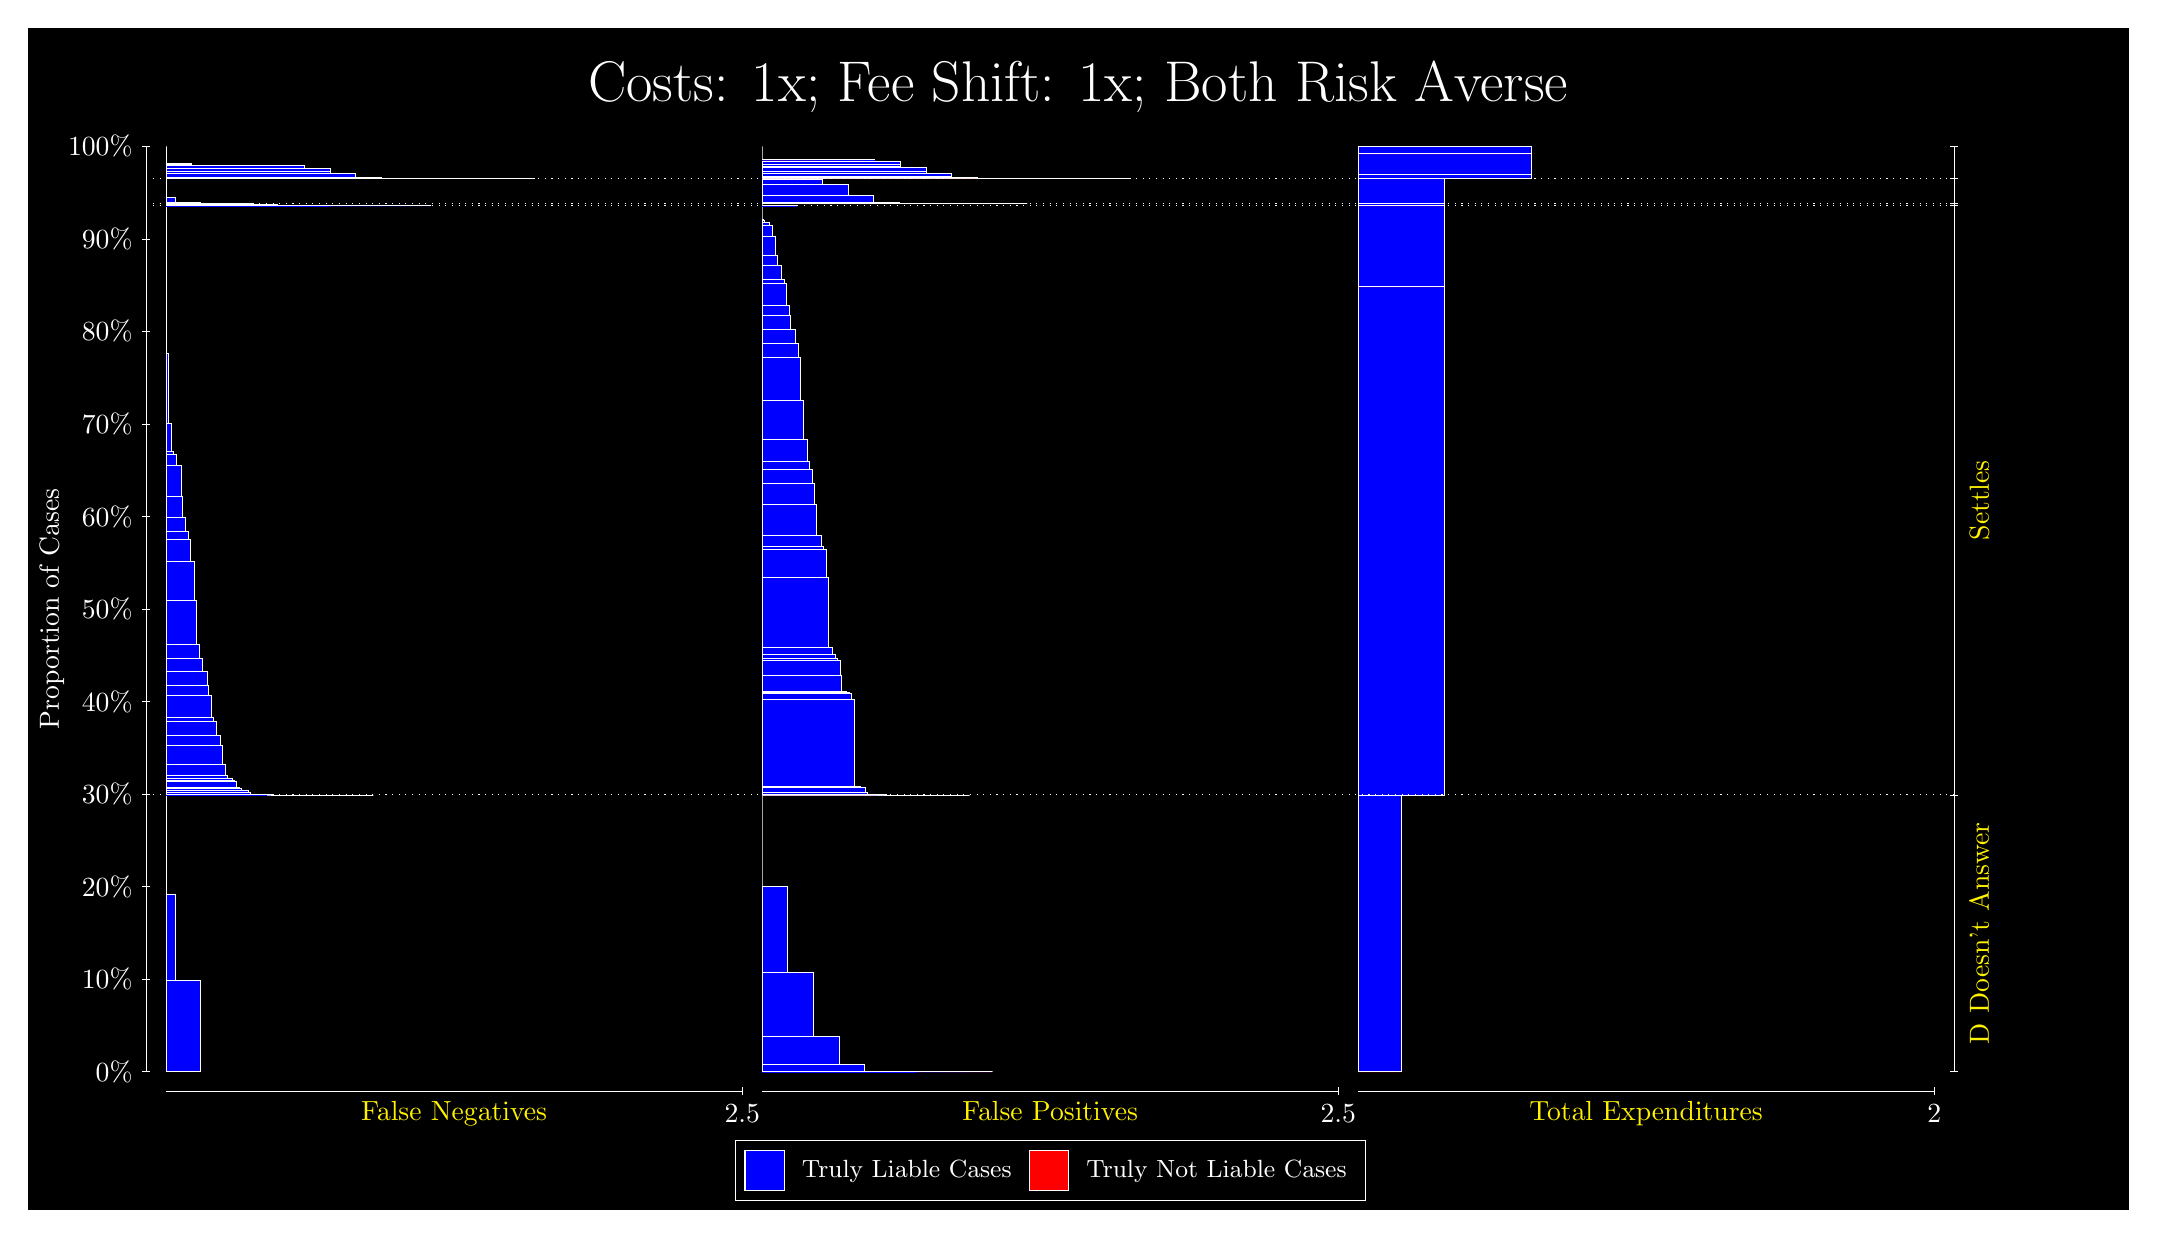
\begin{tikzpicture}
\draw[fill=black] (0,0) rectangle (26.667,15);
\draw[text=white] (0,13.5) rectangle (26.667,15) node[midway] {\huge Costs: 1x; Fee Shift: 1x; Both Risk Averse};
\draw[white, very thin] (1.5,1.75) -- (1.5,13.5);
\node[rotate=90, text=white, anchor=center] at (0.3, 7.625) {Proportion of Cases};
\draw[white, very thin] (1.45,1.75) -- (1.55,1.75);
\node[text=white, anchor=east] at (1.45, 1.75) {0\%};
\draw[white, very thin] (1.45,2.925) -- (1.55,2.925);
\node[text=white, anchor=east] at (1.45, 2.925) {10\%};
\draw[white, very thin] (1.45,4.1) -- (1.55,4.1);
\node[text=white, anchor=east] at (1.45, 4.1) {20\%};
\draw[white, very thin] (1.45,5.275) -- (1.55,5.275);
\node[text=white, anchor=east] at (1.45, 5.275) {30\%};
\draw[white, very thin] (1.45,6.45) -- (1.55,6.45);
\node[text=white, anchor=east] at (1.45, 6.45) {40\%};
\draw[white, very thin] (1.45,7.625) -- (1.55,7.625);
\node[text=white, anchor=east] at (1.45, 7.625) {50\%};
\draw[white, very thin] (1.45,8.8) -- (1.55,8.8);
\node[text=white, anchor=east] at (1.45, 8.8) {60\%};
\draw[white, very thin] (1.45,9.975) -- (1.55,9.975);
\node[text=white, anchor=east] at (1.45, 9.975) {70\%};
\draw[white, very thin] (1.45,11.15) -- (1.55,11.15);
\node[text=white, anchor=east] at (1.45, 11.15) {80\%};
\draw[white, very thin] (1.45,12.325) -- (1.55,12.325);
\node[text=white, anchor=east] at (1.45, 12.325) {90\%};
\draw[white, very thin] (1.45,13.5) -- (1.55,13.5);
\node[text=white, anchor=east] at (1.45, 13.5) {100\%};

\draw[white, very thin] (24.457,1.75) -- (24.457,13.5);
\draw[white, very thin] (24.407,1.75) -- (24.507,1.75);
\node[anchor=west] at (24.407, 1.75) {};
\draw[white, very thin] (24.407,5.264) -- (24.507,5.264);
\node[anchor=west] at (24.407, 5.264) {};
\draw[white, very thin] (24.407,12.745) -- (24.507,12.745);
\node[anchor=west] at (24.407, 12.745) {};
\draw[white, very thin] (24.407,12.779) -- (24.507,12.779);
\node[anchor=west] at (24.407, 12.779) {};
\draw[white, very thin] (24.407,13.095) -- (24.507,13.095);
\node[anchor=west] at (24.407, 13.095) {};
\draw[white, very thin] (24.407,13.5) -- (24.507,13.5);
\node[anchor=west] at (24.407, 13.5) {};

\draw[white, very thin, fill=blue] (1.75,1.75) rectangle (2.1891,2.9145);
\draw[white, very thin, fill=blue] (1.75,2.9145) rectangle (1.8638,4.0054);
\draw[white, very thin, fill=red] (1.75,4.0054) rectangle (1.75,4.0054);
\draw[white, very thin, fill=blue] (1.75,4.0054) rectangle (1.75,5.264);
\draw[white, very thin, fill=blue] (1.75,5.264) rectangle (4.3848,5.264);
\draw[white, very thin, fill=blue] (1.75,5.264) rectangle (4.2384,5.264);
\draw[white, very thin, fill=blue] (1.75,5.264) rectangle (4.092,5.264);
\draw[white, very thin, fill=blue] (1.75,5.264) rectangle (4.0595,5.264);
\draw[white, very thin, fill=blue] (1.75,5.264) rectangle (3.9457,5.264);
\draw[white, very thin, fill=blue] (1.75,5.264) rectangle (3.9131,5.264);
\draw[white, very thin, fill=blue] (1.75,5.264) rectangle (3.7993,5.264);
\draw[white, very thin, fill=blue] (1.75,5.264) rectangle (3.7668,5.264);
\draw[white, very thin, fill=blue] (1.75,5.264) rectangle (3.7342,5.264);
\draw[white, very thin, fill=blue] (1.75,5.264) rectangle (3.6529,5.264);
\draw[white, very thin, fill=blue] (1.75,5.264) rectangle (3.6204,5.264);
\draw[white, very thin, fill=blue] (1.75,5.264) rectangle (3.5878,5.264);
\draw[white, very thin, fill=blue] (1.75,5.264) rectangle (3.5065,5.264);
\draw[white, very thin, fill=blue] (1.75,5.264) rectangle (3.474,5.264);
\draw[white, very thin, fill=blue] (1.75,5.264) rectangle (3.4415,5.264);
\draw[white, very thin, fill=blue] (1.75,5.264) rectangle (3.4089,5.264);
\draw[white, very thin, fill=blue] (1.75,5.264) rectangle (3.3602,5.264);
\draw[white, very thin, fill=blue] (1.75,5.264) rectangle (3.3276,5.264);
\draw[white, very thin, fill=blue] (1.75,5.264) rectangle (3.2951,5.264);
\draw[white, very thin, fill=blue] (1.75,5.264) rectangle (3.2626,5.264);
\draw[white, very thin, fill=blue] (1.75,5.264) rectangle (3.1812,5.2641);
\draw[white, very thin, fill=blue] (1.75,5.2641) rectangle (3.1487,5.2645);
\draw[white, very thin, fill=blue] (1.75,5.2645) rectangle (3.1162,5.265);
\draw[white, very thin, fill=blue] (1.75,5.265) rectangle (3.0837,5.2652);
\draw[white, very thin, fill=blue] (1.75,5.2652) rectangle (3.0349,5.2657);
\draw[white, very thin, fill=blue] (1.75,5.2657) rectangle (3.0023,5.2658);
\draw[white, very thin, fill=blue] (1.75,5.2658) rectangle (2.9698,5.2706);
\draw[white, very thin, fill=blue] (1.75,5.2706) rectangle (2.9373,5.2709);
\draw[white, very thin, fill=blue] (1.75,5.2709) rectangle (2.921,5.2715);
\draw[white, very thin, fill=blue] (1.75,5.2715) rectangle (2.856,5.2737);
\draw[white, very thin, fill=blue] (1.75,5.2737) rectangle (2.8234,5.2926);
\draw[white, very thin, fill=blue] (1.75,5.2926) rectangle (2.7909,5.3174);
\draw[white, very thin, fill=blue] (1.75,5.3174) rectangle (2.7584,5.328);
\draw[white, very thin, fill=blue] (1.75,5.328) rectangle (2.7096,5.3498);
\draw[white, very thin, fill=blue] (1.75,5.3498) rectangle (2.6771,5.3543);
\draw[white, very thin, fill=blue] (1.75,5.3543) rectangle (2.6445,5.4402);
\draw[white, very thin, fill=blue] (1.75,5.4402) rectangle (2.612,5.4538);
\draw[white, very thin, fill=blue] (1.75,5.4538) rectangle (2.5957,5.4727);
\draw[white, very thin, fill=blue] (1.75,5.4727) rectangle (2.5307,5.5172);
\draw[white, very thin, fill=blue] (1.75,5.5172) rectangle (2.4982,5.6533);
\draw[white, very thin, fill=blue] (1.75,5.6533) rectangle (2.4656,5.8966);
\draw[white, very thin, fill=blue] (1.75,5.8966) rectangle (2.4331,6.0253);
\draw[white, very thin, fill=blue] (1.75,6.0253) rectangle (2.3843,6.2028);
\draw[white, very thin, fill=blue] (1.75,6.2028) rectangle (2.3518,6.2518);
\draw[white, very thin, fill=blue] (1.75,6.2518) rectangle (2.3192,6.5329);
\draw[white, very thin, fill=blue] (1.75,6.5329) rectangle (2.2867,6.6548);
\draw[white, very thin, fill=blue] (1.75,6.6548) rectangle (2.2705,6.8272);
\draw[white, very thin, fill=blue] (1.75,6.8272) rectangle (2.2054,7.0046);
\draw[white, very thin, fill=blue] (1.75,7.0046) rectangle (2.1729,7.182);
\draw[white, very thin, fill=blue] (1.75,7.182) rectangle (2.1403,7.7322);
\draw[white, very thin, fill=blue] (1.75,7.7322) rectangle (2.1078,8.2259);
\draw[white, very thin, fill=blue] (1.75,8.2259) rectangle (2.059,8.507);
\draw[white, very thin, fill=blue] (1.75,8.507) rectangle (2.0265,8.6166);
\draw[white, very thin, fill=blue] (1.75,8.6166) rectangle (1.994,8.7941);
\draw[white, very thin, fill=blue] (1.75,8.7941) rectangle (1.9614,9.0561);
\draw[white, very thin, fill=blue] (1.75,9.0561) rectangle (1.9452,9.4475);
\draw[white, very thin, fill=blue] (1.75,9.4475) rectangle (1.8801,9.5835);
\draw[white, very thin, fill=blue] (1.75,9.5835) rectangle (1.8476,9.628);
\draw[white, very thin, fill=blue] (1.75,9.628) rectangle (1.8151,9.9785);
\draw[white, very thin, fill=blue] (1.75,9.9785) rectangle (1.7825,10.875);
\draw[white, very thin, fill=red] (1.75,10.875) rectangle (1.75,10.875);
\draw[white, very thin, fill=blue] (1.75,10.875) rectangle (1.75,12.745);
\draw[white, very thin, fill=blue] (1.75,12.745) rectangle (5.1167,12.745);
\draw[white, very thin, fill=blue] (1.75,12.745) rectangle (4.7914,12.745);
\draw[white, very thin, fill=blue] (1.75,12.745) rectangle (4.4661,12.745);
\draw[white, very thin, fill=blue] (1.75,12.745) rectangle (4.1408,12.745);
\draw[white, very thin, fill=blue] (1.75,12.745) rectangle (3.8155,12.746);
\draw[white, very thin, fill=blue] (1.75,12.746) rectangle (3.4903,12.75);
\draw[white, very thin, fill=blue] (1.75,12.75) rectangle (3.165,12.766);
\draw[white, very thin, fill=blue] (1.75,12.766) rectangle (2.8397,12.777);
\draw[white, very thin, fill=blue] (1.75,12.777) rectangle (2.5144,12.779);
\draw[white, very thin, fill=blue] (1.75,12.779) rectangle (2.1891,12.779);
\draw[white, very thin, fill=red] (1.75,12.779) rectangle (1.75,12.779);
\draw[white, very thin, fill=blue] (1.75,12.779) rectangle (2.1891,12.789);
\draw[white, very thin, fill=blue] (1.75,12.789) rectangle (1.8638,12.849);
\draw[white, very thin, fill=red] (1.75,12.849) rectangle (1.75,12.849);
\draw[white, very thin, fill=blue] (1.75,12.849) rectangle (1.75,13.095);
\draw[white, very thin, fill=blue] (1.75,13.095) rectangle (6.4341,13.095);
\draw[white, very thin, fill=blue] (1.75,13.095) rectangle (6.1088,13.095);
\draw[white, very thin, fill=blue] (1.75,13.095) rectangle (5.7835,13.095);
\draw[white, very thin, fill=blue] (1.75,13.095) rectangle (5.4582,13.095);
\draw[white, very thin, fill=blue] (1.75,13.095) rectangle (5.1329,13.095);
\draw[white, very thin, fill=blue] (1.75,13.095) rectangle (4.8077,13.096);
\draw[white, very thin, fill=blue] (1.75,13.096) rectangle (4.8077,13.098);
\draw[white, very thin, fill=blue] (1.75,13.098) rectangle (4.4824,13.112);
\draw[white, very thin, fill=blue] (1.75,13.112) rectangle (4.4824,13.112);
\draw[white, very thin, fill=blue] (1.75,13.112) rectangle (4.1571,13.156);
\draw[white, very thin, fill=blue] (1.75,13.156) rectangle (3.8318,13.185);
\draw[white, very thin, fill=blue] (1.75,13.185) rectangle (3.8318,13.223);
\draw[white, very thin, fill=blue] (1.75,13.223) rectangle (3.7017,13.223);
\draw[white, very thin, fill=blue] (1.75,13.223) rectangle (3.5065,13.258);
\draw[white, very thin, fill=blue] (1.75,13.258) rectangle (3.3764,13.258);
\draw[white, very thin, fill=blue] (1.75,13.258) rectangle (3.1812,13.26);
\draw[white, very thin, fill=blue] (1.75,13.26) rectangle (3.1812,13.262);
\draw[white, very thin, fill=blue] (1.75,13.262) rectangle (3.1812,13.262);
\draw[white, very thin, fill=blue] (1.75,13.262) rectangle (3.0511,13.262);
\draw[white, very thin, fill=blue] (1.75,13.262) rectangle (3.0511,13.262);
\draw[white, very thin, fill=blue] (1.75,13.262) rectangle (2.856,13.263);
\draw[white, very thin, fill=blue] (1.75,13.263) rectangle (2.856,13.263);
\draw[white, very thin, fill=blue] (1.75,13.263) rectangle (2.7258,13.263);
\draw[white, very thin, fill=blue] (1.75,13.263) rectangle (2.7258,13.263);
\draw[white, very thin, fill=blue] (1.75,13.263) rectangle (2.7258,13.263);
\draw[white, very thin, fill=blue] (1.75,13.263) rectangle (2.5307,13.263);
\draw[white, very thin, fill=blue] (1.75,13.263) rectangle (2.5307,13.263);
\draw[white, very thin, fill=blue] (1.75,13.263) rectangle (2.4006,13.263);
\draw[white, very thin, fill=blue] (1.75,13.263) rectangle (2.4006,13.264);
\draw[white, very thin, fill=blue] (1.75,13.264) rectangle (2.2054,13.264);
\draw[white, very thin, fill=blue] (1.75,13.264) rectangle (2.2054,13.264);
\draw[white, very thin, fill=blue] (1.75,13.264) rectangle (2.0753,13.266);
\draw[white, very thin, fill=blue] (1.75,13.266) rectangle (2.0753,13.271);
\draw[white, very thin, fill=blue] (1.75,13.271) rectangle (2.0753,13.283);
\draw[white, very thin, fill=blue] (1.75,13.283) rectangle (1.8801,13.283);
\draw[white, very thin, fill=blue] (1.75,13.283) rectangle (1.8801,13.283);
\draw[white, very thin, fill=red] (1.75,13.283) rectangle (1.75,13.283);
\draw[white, very thin, fill=blue] (1.75,13.283) rectangle (1.75,13.5);
\draw[white, very thin, fill=red] (9.3189,1.75) rectangle (12.246,1.75);
\draw[white, very thin, fill=blue] (9.3189,1.75) rectangle (12.246,1.75);
\draw[white, very thin, fill=blue] (9.3189,1.75) rectangle (11.921,1.75);
\draw[white, very thin, fill=blue] (9.3189,1.75) rectangle (11.596,1.75);
\draw[white, very thin, fill=blue] (9.3189,1.75) rectangle (11.271,1.7503);
\draw[white, very thin, fill=blue] (9.3189,1.7503) rectangle (10.945,1.7576);
\draw[white, very thin, fill=blue] (9.3189,1.7576) rectangle (10.62,1.8361);
\draw[white, very thin, fill=blue] (9.3189,1.8361) rectangle (10.295,2.1984);
\draw[white, very thin, fill=blue] (9.3189,2.1984) rectangle (9.9694,3.0086);
\draw[white, very thin, fill=blue] (9.3189,3.0086) rectangle (9.6442,4.0995);
\draw[white, very thin, fill=blue] (9.3189,4.0995) rectangle (9.3189,5.264);
\draw[white, very thin, fill=red] (9.3189,5.264) rectangle (11.954,5.264);
\draw[white, very thin, fill=blue] (9.3189,5.264) rectangle (11.954,5.264);
\draw[white, very thin, fill=blue] (9.3189,5.264) rectangle (11.628,5.264);
\draw[white, very thin, fill=red] (9.3189,5.264) rectangle (11.515,5.264);
\draw[white, very thin, fill=blue] (9.3189,5.264) rectangle (11.515,5.264);
\draw[white, very thin, fill=red] (9.3189,5.264) rectangle (11.368,5.264);
\draw[white, very thin, fill=blue] (9.3189,5.264) rectangle (11.368,5.264);
\draw[white, very thin, fill=blue] (9.3189,5.264) rectangle (11.303,5.264);
\draw[white, very thin, fill=red] (9.3189,5.264) rectangle (11.222,5.264);
\draw[white, very thin, fill=blue] (9.3189,5.264) rectangle (11.222,5.264);
\draw[white, very thin, fill=blue] (9.3189,5.264) rectangle (11.189,5.264);
\draw[white, very thin, fill=red] (9.3189,5.264) rectangle (11.075,5.264);
\draw[white, very thin, fill=blue] (9.3189,5.264) rectangle (11.075,5.264);
\draw[white, very thin, fill=blue] (9.3189,5.264) rectangle (11.043,5.264);
\draw[white, very thin, fill=blue] (9.3189,5.264) rectangle (10.978,5.2645);
\draw[white, very thin, fill=red] (9.3189,5.2645) rectangle (10.929,5.2645);
\draw[white, very thin, fill=blue] (9.3189,5.2645) rectangle (10.929,5.2645);
\draw[white, very thin, fill=blue] (9.3189,5.2645) rectangle (10.896,5.2648);
\draw[white, very thin, fill=blue] (9.3189,5.2648) rectangle (10.864,5.2648);
\draw[white, very thin, fill=red] (9.3189,5.2648) rectangle (10.783,5.2648);
\draw[white, very thin, fill=blue] (9.3189,5.2648) rectangle (10.783,5.2754);
\draw[white, very thin, fill=blue] (9.3189,5.2754) rectangle (10.75,5.2754);
\draw[white, very thin, fill=blue] (9.3189,5.2754) rectangle (10.718,5.2759);
\draw[white, very thin, fill=blue] (9.3189,5.2759) rectangle (10.653,5.2987);
\draw[white, very thin, fill=red] (9.3189,5.2987) rectangle (10.636,5.2987);
\draw[white, very thin, fill=blue] (9.3189,5.2987) rectangle (10.636,5.3626);
\draw[white, very thin, fill=blue] (9.3189,5.3626) rectangle (10.604,5.3631);
\draw[white, very thin, fill=blue] (9.3189,5.3631) rectangle (10.571,5.37);
\draw[white, very thin, fill=blue] (9.3189,5.37) rectangle (10.539,5.3747);
\draw[white, very thin, fill=red] (9.3189,5.3747) rectangle (10.49,5.3747);
\draw[white, very thin, fill=blue] (9.3189,5.3747) rectangle (10.49,6.4749);
\draw[white, very thin, fill=blue] (9.3189,6.4749) rectangle (10.457,6.5593);
\draw[white, very thin, fill=blue] (9.3189,6.5593) rectangle (10.425,6.5615);
\draw[white, very thin, fill=blue] (9.3189,6.5615) rectangle (10.392,6.5804);
\draw[white, very thin, fill=blue] (9.3189,6.5804) rectangle (10.327,6.7854);
\draw[white, very thin, fill=blue] (9.3189,6.7854) rectangle (10.311,6.973);
\draw[white, very thin, fill=blue] (9.3189,6.973) rectangle (10.278,6.9948);
\draw[white, very thin, fill=blue] (9.3189,6.9948) rectangle (10.246,7.0489);
\draw[white, very thin, fill=blue] (9.3189,7.0489) rectangle (10.213,7.1348);
\draw[white, very thin, fill=blue] (9.3189,7.1348) rectangle (10.165,8.0308);
\draw[white, very thin, fill=blue] (9.3189,8.0308) rectangle (10.132,8.3814);
\draw[white, very thin, fill=blue] (9.3189,8.3814) rectangle (10.1,8.4259);
\draw[white, very thin, fill=blue] (9.3189,8.4259) rectangle (10.067,8.5619);
\draw[white, very thin, fill=blue] (9.3189,8.5619) rectangle (10.002,8.9533);
\draw[white, very thin, fill=blue] (9.3189,8.9533) rectangle (9.9857,9.2153);
\draw[white, very thin, fill=blue] (9.3189,9.2153) rectangle (9.9532,9.3928);
\draw[white, very thin, fill=blue] (9.3189,9.3928) rectangle (9.9206,9.5024);
\draw[white, very thin, fill=blue] (9.3189,9.5024) rectangle (9.8881,9.7834);
\draw[white, very thin, fill=blue] (9.3189,9.7834) rectangle (9.8393,10.277);
\draw[white, very thin, fill=blue] (9.3189,10.277) rectangle (9.8068,10.827);
\draw[white, very thin, fill=blue] (9.3189,10.827) rectangle (9.7743,11.005);
\draw[white, very thin, fill=blue] (9.3189,11.005) rectangle (9.7417,11.182);
\draw[white, very thin, fill=blue] (9.3189,11.182) rectangle (9.6767,11.355);
\draw[white, very thin, fill=blue] (9.3189,11.355) rectangle (9.6604,11.476);
\draw[white, very thin, fill=blue] (9.3189,11.476) rectangle (9.6279,11.758);
\draw[white, very thin, fill=blue] (9.3189,11.758) rectangle (9.5954,11.807);
\draw[white, very thin, fill=blue] (9.3189,11.807) rectangle (9.5628,11.984);
\draw[white, very thin, fill=blue] (9.3189,11.984) rectangle (9.514,12.113);
\draw[white, very thin, fill=blue] (9.3189,12.113) rectangle (9.4815,12.356);
\draw[white, very thin, fill=blue] (9.3189,12.356) rectangle (9.449,12.492);
\draw[white, very thin, fill=blue] (9.3189,12.492) rectangle (9.4165,12.537);
\draw[white, very thin, fill=blue] (9.3189,12.537) rectangle (9.3514,12.556);
\draw[white, very thin, fill=blue] (9.3189,12.556) rectangle (9.3351,12.569);
\draw[white, very thin, fill=blue] (9.3189,12.569) rectangle (9.3189,12.745);
\draw[white, very thin, fill=red] (9.3189,12.745) rectangle (9.758,12.745);
\draw[white, very thin, fill=blue] (9.3189,12.745) rectangle (9.758,12.746);
\draw[white, very thin, fill=blue] (9.3189,12.746) rectangle (9.4327,12.747);
\draw[white, very thin, fill=blue] (9.3189,12.747) rectangle (9.3189,12.779);
\draw[white, very thin, fill=red] (9.3189,12.779) rectangle (12.686,12.779);
\draw[white, very thin, fill=blue] (9.3189,12.779) rectangle (12.686,12.779);
\draw[white, very thin, fill=blue] (9.3189,12.779) rectangle (12.36,12.779);
\draw[white, very thin, fill=blue] (9.3189,12.779) rectangle (12.035,12.779);
\draw[white, very thin, fill=blue] (9.3189,12.779) rectangle (11.71,12.779);
\draw[white, very thin, fill=blue] (9.3189,12.779) rectangle (11.384,12.779);
\draw[white, very thin, fill=blue] (9.3189,12.779) rectangle (11.059,12.793);
\draw[white, very thin, fill=blue] (9.3189,12.793) rectangle (10.734,12.882);
\draw[white, very thin, fill=blue] (9.3189,12.882) rectangle (10.409,13.024);
\draw[white, very thin, fill=blue] (9.3189,13.024) rectangle (10.083,13.085);
\draw[white, very thin, fill=blue] (9.3189,13.085) rectangle (9.758,13.095);
\draw[white, very thin, fill=red] (9.3189,13.095) rectangle (14.003,13.095);
\draw[white, very thin, fill=blue] (9.3189,13.095) rectangle (14.003,13.095);
\draw[white, very thin, fill=red] (9.3189,13.095) rectangle (13.678,13.095);
\draw[white, very thin, fill=blue] (9.3189,13.095) rectangle (13.678,13.095);
\draw[white, very thin, fill=red] (9.3189,13.095) rectangle (13.352,13.095);
\draw[white, very thin, fill=blue] (9.3189,13.095) rectangle (13.352,13.095);
\draw[white, very thin, fill=blue] (9.3189,13.095) rectangle (13.027,13.095);
\draw[white, very thin, fill=red] (9.3189,13.095) rectangle (13.027,13.095);
\draw[white, very thin, fill=blue] (9.3189,13.095) rectangle (13.027,13.095);
\draw[white, very thin, fill=blue] (9.3189,13.095) rectangle (12.702,13.095);
\draw[white, very thin, fill=red] (9.3189,13.095) rectangle (12.702,13.095);
\draw[white, very thin, fill=blue] (9.3189,13.095) rectangle (12.702,13.095);
\draw[white, very thin, fill=blue] (9.3189,13.095) rectangle (12.377,13.097);
\draw[white, very thin, fill=red] (9.3189,13.097) rectangle (12.377,13.097);
\draw[white, very thin, fill=blue] (9.3189,13.097) rectangle (12.377,13.097);
\draw[white, very thin, fill=blue] (9.3189,13.097) rectangle (12.051,13.101);
\draw[white, very thin, fill=red] (9.3189,13.101) rectangle (12.051,13.101);
\draw[white, very thin, fill=blue] (9.3189,13.101) rectangle (12.051,13.111);
\draw[white, very thin, fill=blue] (9.3189,13.111) rectangle (12.051,13.112);
\draw[white, very thin, fill=blue] (9.3189,13.112) rectangle (12.051,13.112);
\draw[white, very thin, fill=blue] (9.3189,13.112) rectangle (11.726,13.124);
\draw[white, very thin, fill=blue] (9.3189,13.124) rectangle (11.726,13.154);
\draw[white, very thin, fill=blue] (9.3189,13.154) rectangle (11.726,13.157);
\draw[white, very thin, fill=blue] (9.3189,13.157) rectangle (11.401,13.158);
\draw[white, very thin, fill=blue] (9.3189,13.158) rectangle (11.401,13.186);
\draw[white, very thin, fill=blue] (9.3189,13.186) rectangle (11.401,13.239);
\draw[white, very thin, fill=red] (9.3189,13.239) rectangle (11.271,13.239);
\draw[white, very thin, fill=blue] (9.3189,13.239) rectangle (11.271,13.239);
\draw[white, very thin, fill=blue] (9.3189,13.239) rectangle (11.075,13.252);
\draw[white, very thin, fill=blue] (9.3189,13.252) rectangle (11.075,13.273);
\draw[white, very thin, fill=blue] (9.3189,13.273) rectangle (11.075,13.312);
\draw[white, very thin, fill=red] (9.3189,13.312) rectangle (10.945,13.312);
\draw[white, very thin, fill=blue] (9.3189,13.312) rectangle (10.945,13.312);
\draw[white, very thin, fill=blue] (9.3189,13.312) rectangle (10.75,13.317);
\draw[white, very thin, fill=blue] (9.3189,13.317) rectangle (10.75,13.33);
\draw[white, very thin, fill=blue] (9.3189,13.33) rectangle (10.75,13.331);
\draw[white, very thin, fill=blue] (9.3189,13.331) rectangle (10.62,13.331);
\draw[white, very thin, fill=red] (9.3189,13.331) rectangle (10.62,13.331);
\draw[white, very thin, fill=blue] (9.3189,13.331) rectangle (10.62,13.331);
\draw[white, very thin, fill=blue] (9.3189,13.331) rectangle (10.425,13.331);
\draw[white, very thin, fill=blue] (9.3189,13.331) rectangle (10.425,13.332);
\draw[white, very thin, fill=blue] (9.3189,13.332) rectangle (10.295,13.332);
\draw[white, very thin, fill=red] (9.3189,13.332) rectangle (10.295,13.332);
\draw[white, very thin, fill=blue] (9.3189,13.332) rectangle (10.295,13.332);
\draw[white, very thin, fill=blue] (9.3189,13.332) rectangle (10.1,13.332);
\draw[white, very thin, fill=blue] (9.3189,13.332) rectangle (10.1,13.332);
\draw[white, very thin, fill=blue] (9.3189,13.332) rectangle (10.1,13.332);
\draw[white, very thin, fill=blue] (9.3189,13.332) rectangle (9.9694,13.332);
\draw[white, very thin, fill=red] (9.3189,13.332) rectangle (9.9694,13.332);
\draw[white, very thin, fill=blue] (9.3189,13.332) rectangle (9.9694,13.332);
\draw[white, very thin, fill=blue] (9.3189,13.332) rectangle (9.7743,13.332);
\draw[white, very thin, fill=blue] (9.3189,13.332) rectangle (9.7743,13.332);
\draw[white, very thin, fill=blue] (9.3189,13.332) rectangle (9.6442,13.332);
\draw[white, very thin, fill=red] (9.3189,13.332) rectangle (9.6442,13.332);
\draw[white, very thin, fill=blue] (9.3189,13.332) rectangle (9.6442,13.335);
\draw[white, very thin, fill=blue] (9.3189,13.335) rectangle (9.6442,13.337);
\draw[white, very thin, fill=blue] (9.3189,13.337) rectangle (9.449,13.337);
\draw[white, very thin, fill=blue] (9.3189,13.337) rectangle (9.449,13.337);
\draw[white, very thin, fill=red] (9.3189,13.337) rectangle (9.3189,13.337);
\draw[white, very thin, fill=blue] (9.3189,13.337) rectangle (9.3189,13.5);
\draw[white, very thin, fill=red] (16.888,1.75) rectangle (17.437,1.75);
\draw[white, very thin, fill=blue] (16.888,1.75) rectangle (17.437,5.264);
\draw[white, very thin, fill=red] (16.888,5.264) rectangle (17.986,5.264);
\draw[white, very thin, fill=blue] (16.888,5.264) rectangle (17.986,11.717);
\draw[white, very thin, fill=red] (16.888,11.717) rectangle (17.986,11.717);
\draw[white, very thin, fill=blue] (16.888,11.717) rectangle (17.986,12.745);
\draw[white, very thin, fill=red] (16.888,12.745) rectangle (17.986,12.745);
\draw[white, very thin, fill=blue] (16.888,12.745) rectangle (17.986,12.779);
\draw[white, very thin, fill=red] (16.888,12.779) rectangle (17.986,12.779);
\draw[white, very thin, fill=blue] (16.888,12.779) rectangle (17.986,13.095);
\draw[white, very thin, fill=red] (16.888,13.095) rectangle (19.083,13.095);
\draw[white, very thin, fill=blue] (16.888,13.095) rectangle (19.083,13.146);
\draw[white, very thin, fill=red] (16.888,13.146) rectangle (19.083,13.146);
\draw[white, very thin, fill=blue] (16.888,13.146) rectangle (19.083,13.408);
\draw[white, very thin, fill=red] (16.888,13.408) rectangle (19.083,13.408);
\draw[white, very thin, fill=blue] (16.888,13.408) rectangle (19.083,13.5);
\draw[white, dotted] (1.5,5.264) -- (24.457,5.264);
\draw[white, dotted] (1.5,12.745) -- (24.457,12.745);
\draw[white, dotted] (1.5,12.779) -- (24.457,12.779);
\draw[white, dotted] (1.5,13.095) -- (24.457,13.095);
\draw[white, very thin] (1.75,1.5) -- (9.0689,1.5);
\node[text=yellow, anchor=north] at (5.4094, 1.5) {False Negatives};
\draw[white, very thin] (9.0689,1.45) -- (9.0689,1.55);
\node[text=white, anchor=north] at (9.0689, 1.45) {2.5};

\draw[white, very thin] (9.3189,1.5) -- (16.638,1.5);
\node[text=yellow, anchor=north] at (12.978, 1.5) {False Positives};
\draw[white, very thin] (16.638,1.45) -- (16.638,1.55);
\node[text=white, anchor=north] at (16.638, 1.45) {2.5};

\draw[white, very thin] (16.888,1.5) -- (24.207,1.5);
\node[text=yellow, anchor=north] at (20.547, 1.5) {Total Expenditures};
\draw[white, very thin] (24.207,1.45) -- (24.207,1.55);
\node[text=white, anchor=north] at (24.207, 1.45) {2};

\node[text=yellow, centered, rotate=90] at (24.777, 3.507) {D Doesn't Answer};
\node[text=yellow, centered, rotate=90] at (24.777, 9.0047) {Settles};




\draw (12.978300999999998,1.5) node[draw=none] (baseCoordinate) {};
\begin{scope}[align=center]
        \matrix[scale=0.5, draw=white, below=0.5cm of baseCoordinate, nodes={draw}, column sep=0.1cm]{
            \node[rectangle, draw, minimum width=0.5cm, minimum height=0.5cm, fill=blue] {}; &
            \node[draw=none, font=\small, text=white] (B) {Truly Liable Cases}; &
            \node[rectangle, draw, minimum width=0.5cm, minimum height=0.5cm, fill=red] {}; &
            \node[draw=none, font=\small, text=white] (B) {Truly Not Liable Cases}; \\
            };
\end{scope}

\end{tikzpicture}
\end{document}